\documentclass[]{book}
\usepackage{lmodern}
\usepackage{amssymb,amsmath}
\usepackage{ifxetex,ifluatex}
\usepackage{fixltx2e} % provides \textsubscript
\ifnum 0\ifxetex 1\fi\ifluatex 1\fi=0 % if pdftex
  \usepackage[T1]{fontenc}
  \usepackage[utf8]{inputenc}
\else % if luatex or xelatex
  \ifxetex
    \usepackage{mathspec}
  \else
    \usepackage{fontspec}
  \fi
  \defaultfontfeatures{Ligatures=TeX,Scale=MatchLowercase}
\fi
% use upquote if available, for straight quotes in verbatim environments
\IfFileExists{upquote.sty}{\usepackage{upquote}}{}
% use microtype if available
\IfFileExists{microtype.sty}{%
\usepackage{microtype}
\UseMicrotypeSet[protrusion]{basicmath} % disable protrusion for tt fonts
}{}
\usepackage[margin=1in]{geometry}
\usepackage{hyperref}
\hypersetup{unicode=true,
            pdftitle={Quantitative Human Physiology},
            pdfauthor={Jeffrey A. Walker},
            pdfborder={0 0 0},
            breaklinks=true}
\urlstyle{same}  % don't use monospace font for urls
\usepackage{natbib}
\bibliographystyle{apalike}
\usepackage{longtable,booktabs}
\usepackage{graphicx,grffile}
\makeatletter
\def\maxwidth{\ifdim\Gin@nat@width>\linewidth\linewidth\else\Gin@nat@width\fi}
\def\maxheight{\ifdim\Gin@nat@height>\textheight\textheight\else\Gin@nat@height\fi}
\makeatother
% Scale images if necessary, so that they will not overflow the page
% margins by default, and it is still possible to overwrite the defaults
% using explicit options in \includegraphics[width, height, ...]{}
\setkeys{Gin}{width=\maxwidth,height=\maxheight,keepaspectratio}
\IfFileExists{parskip.sty}{%
\usepackage{parskip}
}{% else
\setlength{\parindent}{0pt}
\setlength{\parskip}{6pt plus 2pt minus 1pt}
}
\setlength{\emergencystretch}{3em}  % prevent overfull lines
\providecommand{\tightlist}{%
  \setlength{\itemsep}{0pt}\setlength{\parskip}{0pt}}
\setcounter{secnumdepth}{5}
% Redefines (sub)paragraphs to behave more like sections
\ifx\paragraph\undefined\else
\let\oldparagraph\paragraph
\renewcommand{\paragraph}[1]{\oldparagraph{#1}\mbox{}}
\fi
\ifx\subparagraph\undefined\else
\let\oldsubparagraph\subparagraph
\renewcommand{\subparagraph}[1]{\oldsubparagraph{#1}\mbox{}}
\fi

%%% Use protect on footnotes to avoid problems with footnotes in titles
\let\rmarkdownfootnote\footnote%
\def\footnote{\protect\rmarkdownfootnote}

%%% Change title format to be more compact
\usepackage{titling}

% Create subtitle command for use in maketitle
\providecommand{\subtitle}[1]{
  \posttitle{
    \begin{center}\large#1\end{center}
    }
}

\setlength{\droptitle}{-2em}

  \title{Quantitative Human Physiology}
    \pretitle{\vspace{\droptitle}\centering\huge}
  \posttitle{\par}
    \author{Jeffrey A. Walker}
    \preauthor{\centering\large\emph}
  \postauthor{\par}
      \predate{\centering\large\emph}
  \postdate{\par}
    \date{2019-04-01}

\usepackage{booktabs}
\usepackage{amsthm}
\makeatletter
\def\thm@space@setup{%
  \thm@preskip=8pt plus 2pt minus 4pt
  \thm@postskip=\thm@preskip
}
\makeatother

\begin{document}
\maketitle

{
\setcounter{tocdepth}{1}
\tableofcontents
}
\chapter*{Directions}\label{directions}
\addcontentsline{toc}{chapter}{Directions}

\begin{enumerate}
\def\labelenumi{\arabic{enumi}.}
\item
  Create a Google Sheets file that you will share with me. Name the
  sheet ``last name BIO 223'', for example ``Walker BIO 223''
\item
  Create one sheet for each assignment. There are 10 assignments so your
  document should have 10 sheets.
\item
  Name each sheet using the assignment name. For example ``1. Blood'',
  ``2. Immune'', etc.
\end{enumerate}

Do not create ten separate Google Sheets files. Do not spread a single
assignment over multiple sheets.

\chapter{Blood}\label{blood}

Goals: back-of-the-envelope estimation, scale, google search

Many complex problems in biology can be broken down into a series of
smaller problems and a common smaller problem is the \textbf{estimation}
of some number, such as the number of bacteria per cell. Estimation
problems range from \textbf{back-of-the-envelope estimations} that are
imprecise but useful in that they give one a general sense of the
\textbf{magnitude} of a phenomenon to more precisely modeled estimates
that are used for making \textbf{decisions under uncertainty}.
Back-of-the-envelope estimations are called that because most can,
literally, be done with a pencil and the back of an envelope. They can
be done with pencil because the computations uses rounded instead of
exact numbers like 10 or 300 that are easily multiplied/divided. In this
module, you will compute some back-of-the-envelope estimations.

A problem like ``how many bacteria can colonize a cell'' depends on the
distribution of the sizes of the bacteria, the size of the cell, and how
packed the cell is with its own molecules and organelles. Here, I simply
want to get you started on addressing a problem like this with very
simple models of the problem. Along the way, solving the problem should
give you a sense of scale of what it is like to be a bacterium or a
virus living in a cellular world.

\section{How to solve an estimation
problem}\label{how-to-solve-an-estimation-problem}

I'll solve an analogous problem: How many beach balls can fit in a barn?
If a barn has Volume \(V_{barn}\) and a beach ball has volume
\(V_{ball}\) then the number of balls that could fit into the barn would
be approximately, \(N_{balls} = \frac{V_{barn}}{V_{ball}}\). To solve
this, I need to \textbf{paramaterize the model} by assigning numbers to
these variables. And, the answer is dependent on what numbers I choose
for the size of the beach balls and the shape and size of the barn and
how filled the barn is with hay (or furniture or horses or whatever) --
that is how much of the volume of the barn is available for beach balls.
A back-of-the-envelope calculation simply uses a \emph{reasonable} value
for the parameters. So, here are my numbers.

\begin{enumerate}
\def\labelenumi{\arabic{enumi}.}
\tightlist
\item
  the barn is a typical vermont barn. I have a sense of what ``typical''
  is because I live in New England and see barns every day. But what if
  I were a martian, and had never seen a barn? Then I would need to find
  this information from a reliable source. So, to find ``typical'', I
  used a google search and found what looks like a reputable source that
  says a typical hay barn is 30 feet wide by 40 feet long. I estimated
  wall height from the figure as half the width and I used a 12/12 pitch
  for the roof, so the peak is centered and 15 feet (half of the width)
  high.
\end{enumerate}

Again -- if you don't have to look up information to parameterize your
model, don't!

\begin{enumerate}
\def\labelenumi{\arabic{enumi}.}
\setcounter{enumi}{1}
\item
  I used a big beach ball of 2 feet in diameter (because big beach balls
  are fun). I didn't need to look this up!
\item
  10\% of the barn is filled with hay.
\end{enumerate}

I use Google Sheets to compute the number of balls for each room (the
main room and the attic) and then add these. Here is my sheet

\begin{figure}

{\centering 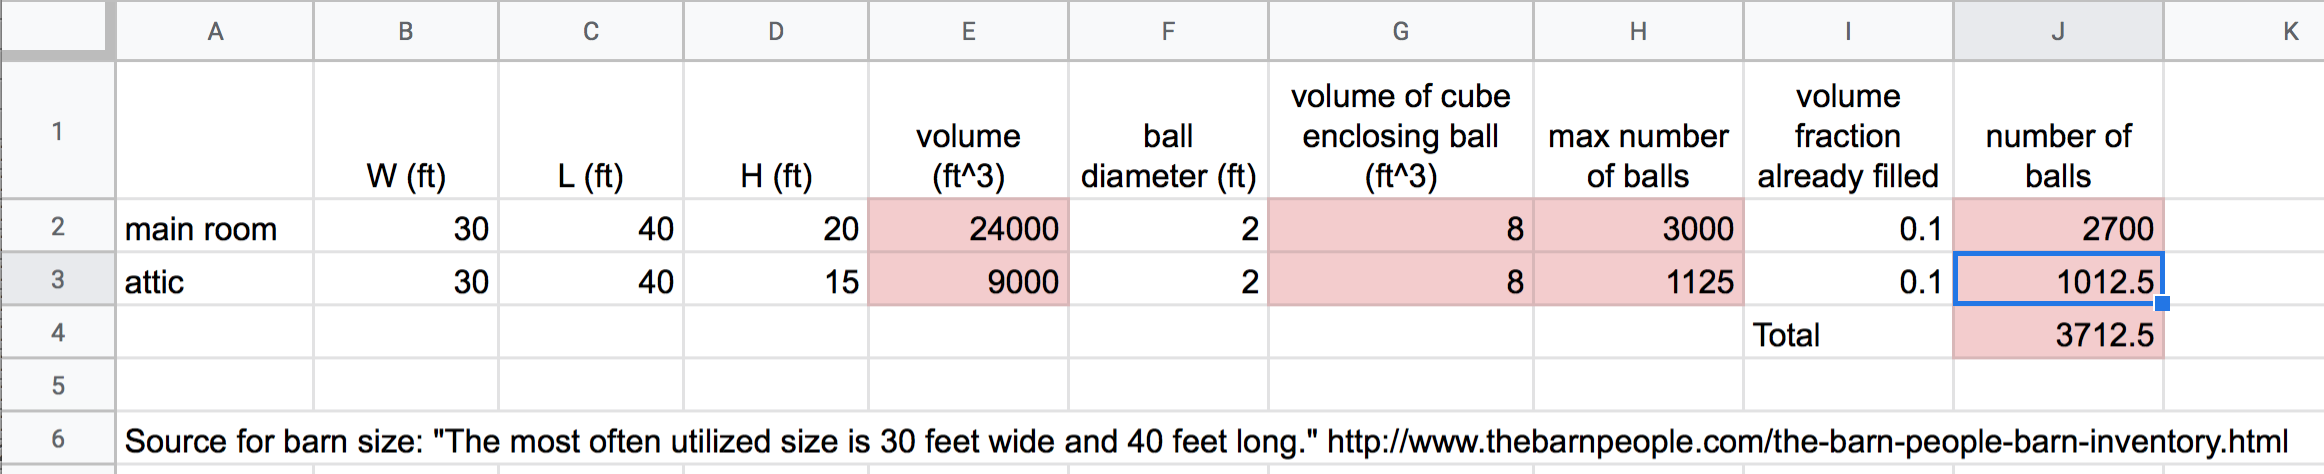
\includegraphics[width=0.8\linewidth]{images/balls} 

}

\caption{Estimation of maximum number of beach balls that could colonize a barn. Cells in red are computed.}\label{fig:balls}
\end{figure}

My column labels include the units of the measure. \textbf{Do not add
units to the measure itself} because this makes the format of the cell
``text'' instead of ``number'' and you cannot refer to the cell in an
equation. I also cite the source of the parameterization below the table
(I cite the source for the size of the barn. The size of the beach ball
I just made up).

\section{Problem set}\label{problem-set}

Do these on the same sheet. Name the sheet ``1. Blood''.

\begin{enumerate}
\def\labelenumi{\arabic{enumi}.}
\tightlist
\item
  How many red blood cells in a drop of blood? Note, I don't want you to
  look up how many RBCs are in a drop, I want you to estimate it using a
  back-of-the-envelope estimation. You don't need to look up the volume
  of a drop of water if you are able to use available information in
  your head to derive a reasonable volume for a drop of water.
\end{enumerate}

For the next three questions, assume the host cell is ``empty'', that
is, it contains no organelles or molecules that take up space.

\begin{enumerate}
\def\labelenumi{\arabic{enumi}.}
\setcounter{enumi}{1}
\item
  How many bacteria could colonize a red blood cell?
\item
  How many bacteria could colonize a macrophage?
\item
  How many virus particles could colonize a red blood cell?
\end{enumerate}

-- These should all be on the same google sheet.

-- \textbf{Do not hardcode parameters}, that is, if a virus is 30 feet
wide do not put ``30'' in an equation but instead make your equations
reference the cell with this information.

-- You may need to google search information to parameterize the model,
such as, how big a virus is. Part of the goal of this is for you to
develop your skills finding reliable information using a google search.
There is variation in virus size or cell size so use something in the
middle or ``typical''. Again -- these are back-of-the-envelope estimates
so you don't need to be very precise -- in fact all of these problems
could be computed by most working biologists without looking up any
information. We all have a pretty good sense for how big a virus, a
bacterium, a blood cell, and a drop of water is. But you can look up
this information because you are at the beginning of your biology
career.

-- Cite a webpage giving the source of the information, as I've done for
the barns. There is no ``right'' or ``wrong'' place to get this
information, only more or less reliable. I'm not grading you on where
you get it, but I want to see where you get it! And all I want for a
citation is the webpage, this is not a formal citation that you put in a
scientific paper.

\chapter{Immune}\label{immune}

Goals: combinations

How many kinds of antibody can a human make by V(D)J recombination?

An individual human produces many different antibody proteins, where
``different'' is amino acid sequence. How is this possible given that
there are only a few ``antibody'' genes? Part of the answer is V(D)J
recombination. An antibody is constructed from two pairs of
polypeptides. Each pair consists of a light chain and a heavy chain.
Each chain has a ``variable'' region and a ``constant'' region. The
heavy chain is constructed from one gene (located on chromosome 14)
while the light chain is constructed from two genes: the light chain
locus \(\lambda\) (``lambda'') located on chromosome 22 and the light
chain locus \(\kappa\) (``kappa'') located on chromosome 2. The variable
region of both light chain loci is composed of a V part and a J part.
The variable region of the heavy chain locus is composed of V, D, and J
parts. A V, D, or J part consists of multiple copies of the exon that
will be spliced into the mRNA but each of these copies has a slightly
different nucleotide sequence and some of the copies do not produce
functional mRNA.

To make the heavy chain mRNA for the antibody

\begin{enumerate}
\def\labelenumi{\arabic{enumi}.}
\item
  Choose one of the copies of the V region of the heavy chain locus.
\item
  Choose one of the copies of the D region of the heavy chain locus.
\item
  Choose one of the copies of the J region of the heavy chain locus.
\end{enumerate}

combine with the C (constant) region to make the heavy chain mRNA

To make the light chain mRNA for the antibody

\begin{enumerate}
\def\labelenumi{\arabic{enumi}.}
\item
  Choose one of the copies of the V region of one (either \(\lambda\) or
  \(\kappa\)) light chain locus.
\item
  Choose one of the copies of the J region of the same light chain
  locus.
\end{enumerate}

combine with the C region to make the light chain mRNA.

Finally, combine the light and heavy chains (these are actually
translated independently and then joined into the protein but the math
is the same).

So an antibody is a combination of combinations. It is a combination
(light + heavy combined) of combinations (V, J, and D combined)

\section{Combinations}\label{combinations}

If there are n1 elements in set 1 and n2 elements in set 2, how many
combinations of 1 element of each set are there? Answer: n1 x n2

In the table below, I use this math to compute the number of antibodies
that could be made using only V(D)J recombination. The

\begin{figure}

{\centering 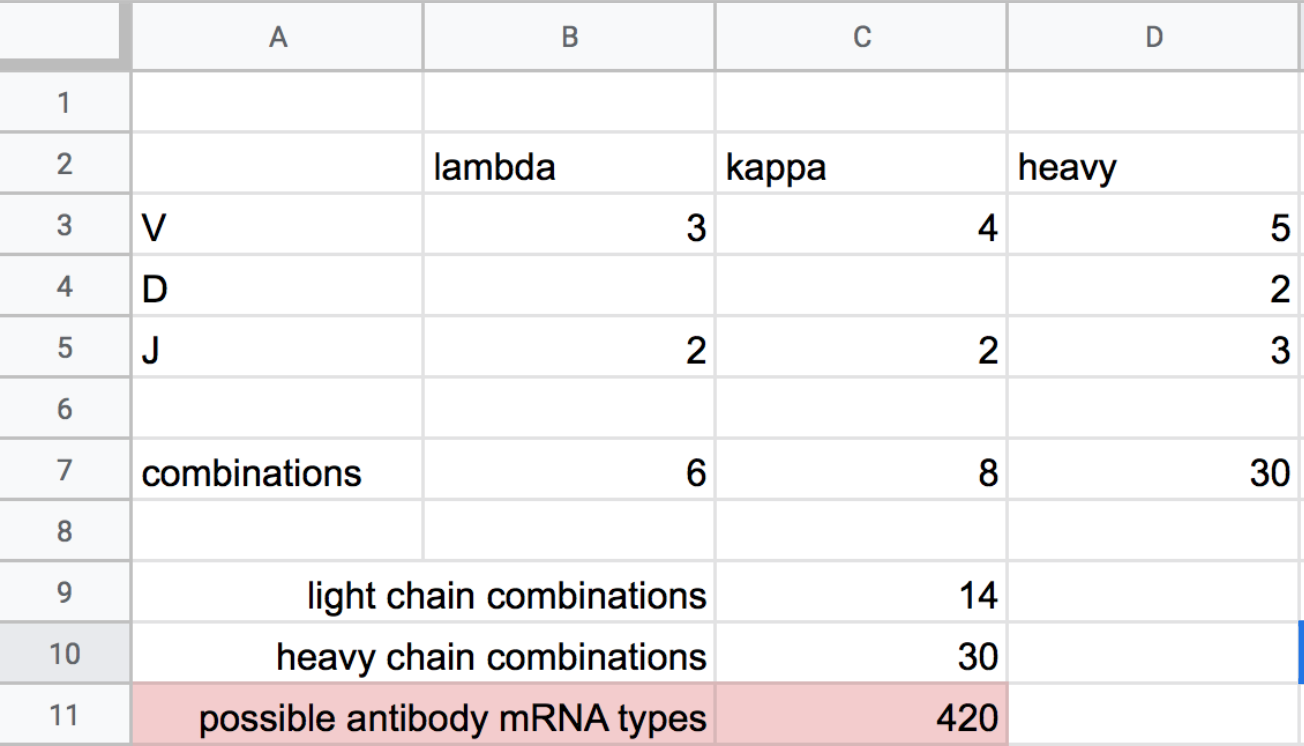
\includegraphics[width=0.8\linewidth]{images/vdj} 

}

\caption{How many kinds of antibodies}\label{fig:vdj}
\end{figure}

\section{Problem set}\label{problem-set-1}

Do these on the same sheet. Name the sheet ``2. Immune''

\begin{enumerate}
\def\labelenumi{\arabic{enumi}.}
\item
  (Ken, Jeff, David, and Doug) is the set of male faculty members in the
  Biology department. (Chris, Terry, Rachel1, Rachel2, and Rachel3) is
  the set of female faculty members in the Biology department. If the
  biology department has a square dance, how many combinations of
  male-female partners could there be? Write all of these out to confirm
  (write this in a column of your google sheet)
\item
  Figure 4.3 in this
  \href{https://www.ncbi.nlm.nih.gov/books/NBK27140/}{online textbook}
  is a table containing the number of copies of each of the gene
  segments. Use this table to compute the number of different antibodies
  that can be synthesized using V(D)J recombination alone.
\end{enumerate}

\chapter{Cardiovascular}\label{cardiovascular}

\section{Background}\label{background}

This exercise explores equations 12-1 and 12-2 from Vander's Physiology.

Regulation of blood flow is critical to increase or decrease delivery of
blood to organs as they need more or less blood. Blood flow can be
modeled with the equation for fluid flow used in almost any system
(rivers, wind, etc)

\begin{equation}
F = \frac{\Delta P}{R} \quad \small{(12.1)}
\end{equation}

\begin{enumerate}
\def\labelenumi{\arabic{enumi}.}
\tightlist
\item
  \(F\) is flow
\item
  \(P\) is pressure. Here, and almost everywhere you'll see it,
  \(\Delta\) (the greek letter ``delta'') means ``change'', so
  \(\Delta P\) (``delta p'') is a \emph{difference} in pressure between
  two points in space. Here this is two points along the length of a
  blood vessel. It is the difference in pressure that is driving the
  blood to flow.
\item
  \(R\) is the resistance to flow due to friction. Friction sucks
  kinetic energy from moving objects (the lost kinetic energy is
  transformed to heat).
\end{enumerate}

Resistance is an important concept in understanding human physiology.
Resistance can be modeled using the Poiseuille equation

\begin{equation}
R = \frac{8L\eta}{\pi r^4} \quad \small{(12.2)}
\end{equation}

\begin{enumerate}
\def\labelenumi{\arabic{enumi}.}
\tightlist
\item
  \(L\) is the length of section of blood vessel
\item
  \(\eta\) (the greek letter ``eta'') is the viscosity of the fluid (or
  more specifically, the dynamic viscosity)
\item
  \(r\) is the radius of the lumen of the vessel.
\end{enumerate}

\section{Problems}\label{problems}

Create a sheet named ``3. cardiovascular''

\begin{enumerate}
\def\labelenumi{\arabic{enumi}.}
\tightlist
\item
  Create a table like that below. Write down the units of each of the
  terms. There is no ``right'' answer, because units can be written
  different ways. For example I could write the units of volume as L
  (``liter'') or gallon or L\(^3\) (here ``L'' is length). Write down a
  definition of each term. Write a formal definition and then add your
  own interpretation of that definition. For example, Wikipedia defines
  density as the ``mass per unit volume'' which I'll interpret as ``the
  amount of matter in given amount of space'', which doesn't quite
  capture the nuances but is helpful for understanding. Also notice that
  wikipedia's definition of density here is an equation expressed as
  words, this can help with thinking about units.
\end{enumerate}

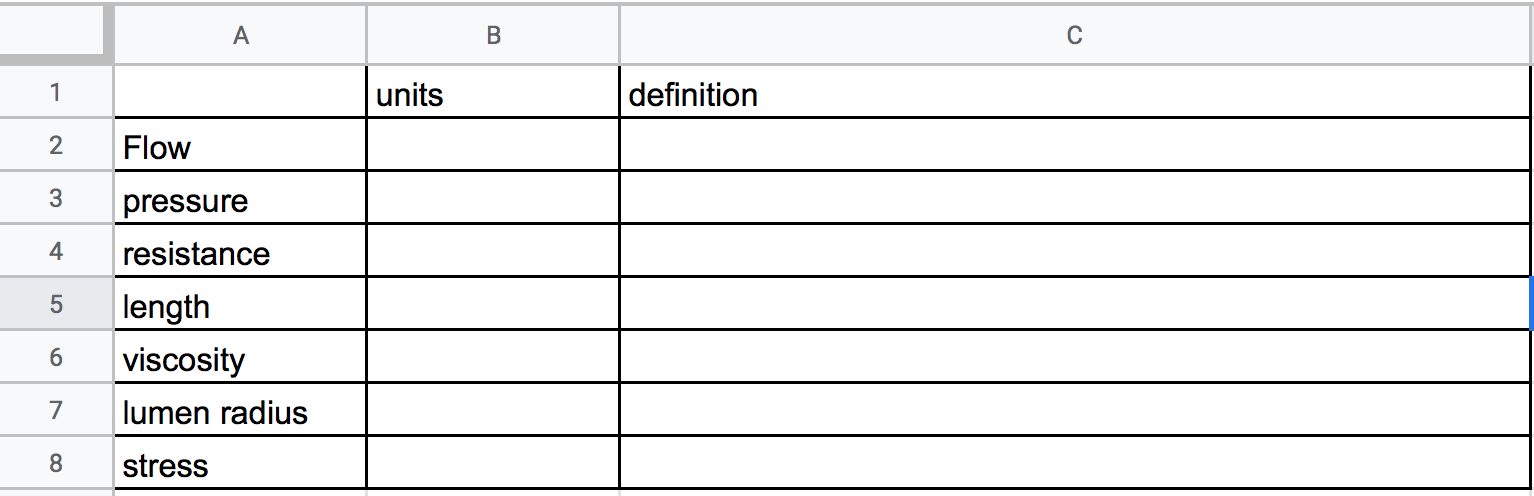
\includegraphics{images/flow_table.png}

\begin{enumerate}
\def\labelenumi{\arabic{enumi}.}
\setcounter{enumi}{1}
\tightlist
\item
  The typical units of viscosity, \(\mathrm{Pa}\cdot \mathrm{s}\) is not
  very intuitive. Wikipedia gives a nice way to think about viscosity:
\end{enumerate}

\begin{quote}
Viscosity is the material property which relates the viscous stresses in
a material to the rate of change of a deformation (the strain rate)
\end{quote}

Using your knowledge of stress and strain from last semester, how would
you express this in units? To answer this 1) write
``Viscosity\ldots{}relates the viscous stresses in a material to the
rate of change of a deformation'' as an equation, and then 2) determine
the units from this equation. Show how the units expressed this way
equals \(\mathrm{Pa}\cdot \mathrm{s}\). Do this with pencil and paper,
snap a photo, and insert it below the table in your Google sheet.

Here is an example to follow: While the equation for flow is useful for
understanding how variation in pressure and resistance cause variation
in flow, if I use the equation to define flow, I would get something
like ``the change in pressure of the fluid per unit resistance'', which
isn't very helpful in thinking about flow. Flow is ``the volume of fluid
that moves past a point per unit time''. So how do I get from the
equation to this definition? I worked this out, snapped a photo,
re-sized the image to 800 pixels wide, then inserted the image in my
google sheet.

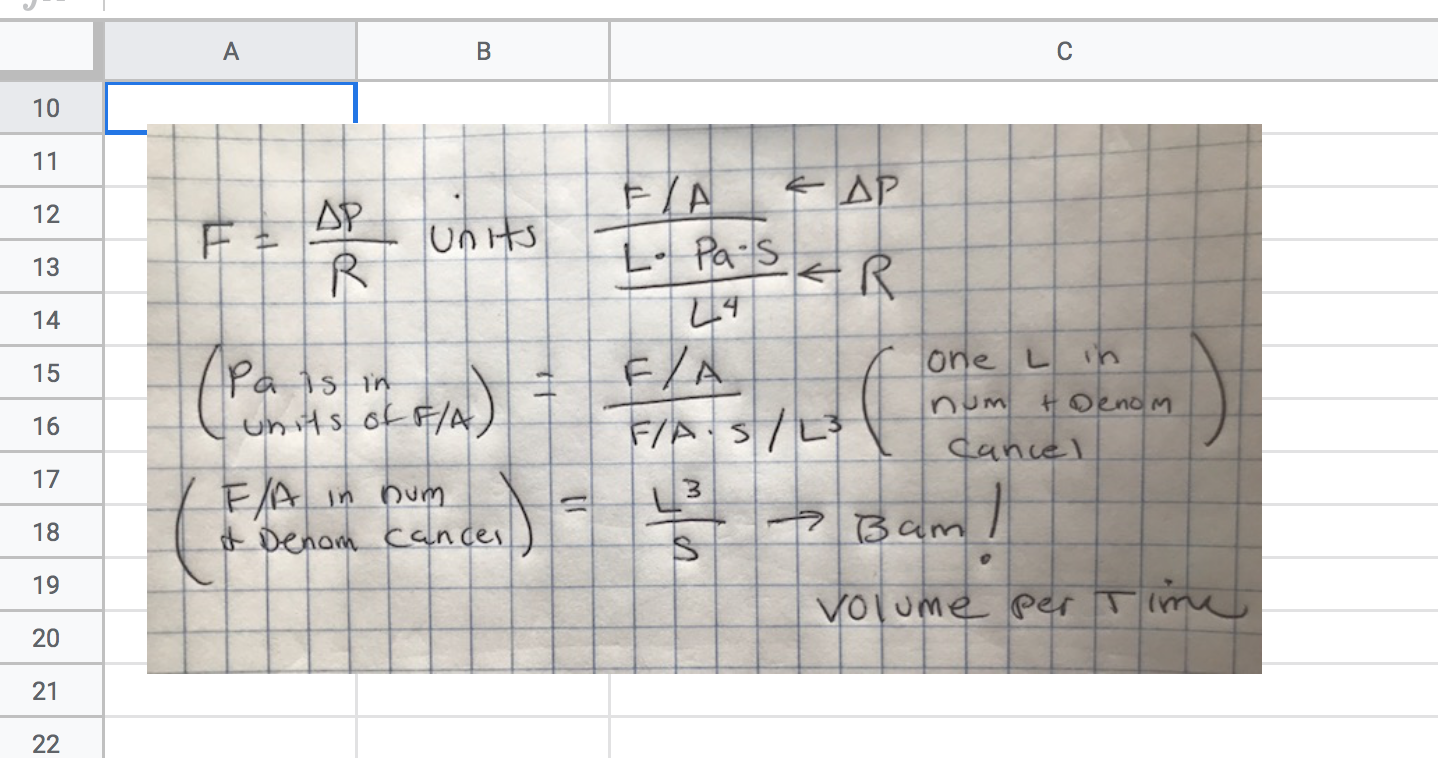
\includegraphics{images/flow-units.png}

\begin{enumerate}
\def\labelenumi{\arabic{enumi}.}
\setcounter{enumi}{2}
\tightlist
\item
  The radius of the lumen of an arteriole leading into a capilary
  increases 50\%. What is the change in blood flow to the capillary? Use
  the google sheet to show your work, including \emph{all} calculations.
\end{enumerate}

\chapter{Resipiratory -- Why we need
Hemoglobin}\label{resipiratory-why-we-need-hemoglobin}

We need hemoglobin because our blood cannot carry enough dissolved O2 to
support our cell activity. That's the short answer. Let's explore a
quantitative answer.

\section{How much O2 can dissolve into
blood?}\label{how-much-o2-can-dissolve-into-blood}

We can model what is going on in the alveoli using a beaker filled with
water. Diffusion of gas molecules from the air into the water (``going
into solution'') or the reverse (``coming out of solution'') is not
simply a function of the concentration gradient of the gas between the
air and the water because \emph{gasses have different solubilities in
solution}.

Equilibrium (when an equal amount of gas is going into and out of
solution) is modeled by the following equation

\begin{equation}
c_\mathrm{O_2} = h_\mathrm{O_2} P_\mathrm{O_2}
\end{equation}

\begin{itemize}
\tightlist
\item
  \(c_\mathrm{O_2}\) is the concentration of O2 in the water
\item
  \(P_\mathrm{O_2}\) is the partial pressure of O2 in air (so a measure
  of concentration)
\item
  \(h_\mathrm{O_2}\) is Henry's solubility coefficient (or ``constant of
  proportionality'').
\end{itemize}

Scientists in different fields have different ways of expressing the
relationship between \(c_\mathrm{O_2}\) and \(P_\mathrm{O_2}\) so you
may land on a web page or a textbook that expresses the constant in
something like \(\frac{1}{c_\mathrm{O_2}}\) or even a dimensionless
constant. I like this way for physiology because it pumps our intuition
about how \(P_\mathrm{O_2}\) controls our dissolved O2 levels.

This equation tells us how much O2 will dissolve in the water at
different partial pressures of O2 in the air, or, switching back to the
lung, how much O2 will dissolve in the blood plasma given the partial
pressure of O2 in the alveolar air.

Below is a table of \(P_\mathrm{O_2}\) of alveolar air and the resulting
concentration of dissolved O2 at equilibrium.

\begin{tabular}{r|r}
\hline
P\_O2 (mmHg) & c\_O2 (mL O2/dL blood)\\
\hline
20 & 0.066\\
\hline
30 & 0.091\\
\hline
40 & 0.137\\
\hline
50 & 0.156\\
\hline
60 & 0.195\\
\hline
70 & 0.220\\
\hline
80 & 0.257\\
\hline
90 & 0.281\\
\hline
100 & 0.307\\
\hline
110 & 0.349\\
\hline
\end{tabular}

\begin{enumerate}
\def\labelenumi{\arabic{enumi}.}
\item
  Transfer the data into your spreadsheet.
\item
  Plot \(c_\mathrm{O_2}\) (y-axis) against \(P_\mathrm{O_2}\) (x-axis)
\item
  Compute the slope and and in the cell next to the computation, write
  the units.
\item
  What is this slope? (the concept not the value)
\item
  What is \(c_\mathrm{O_2}\) in healthy arterial blood entering an organ
  (use \(P_\mathrm{O_2} = 97\) mmHg)?
\item
  How much dissolved O2 is ejected from our left ventricle each minute?
  Again, use \(P_\mathrm{O_2} = 97\) mmHg
\item
  How much O2 do our tissues need each minute? For this, you need to
  look up resting O2 consumption, which is usually in units of mL O2 per
  min per Kg. From this, you use the mass of a person to compute their
  O2 consumption per minute.
\item
  Compare the dissolved O2 sent by the left ventricle to the O2 required
  at rest? Do we send enough dissolvd O2 to our tissues?
\end{enumerate}

\chapter{Renal}\label{renal}

\section{A back of the envelope calculation of
GFR}\label{a-back-of-the-envelope-calculation-of-gfr}

\begin{enumerate}
\def\labelenumi{\arabic{enumi}.}
\tightlist
\item
  Estimate GFR using a back-of-the-envelope calculation. The calculation
  is
\end{enumerate}

GFR = cardiac output X renal fraction X plasma fraction X filtration
fraction

Look up reasonable values for the four variables to parameterize this
equation. Do the computation in your Google Sheet. Insert the units of
GFR in the adjacent cell.

\section{Using renal clearance to measure GFR in an
indivudal}\label{using-renal-clearance-to-measure-gfr-in-an-indivudal}

\begin{equation}
C_s = \frac{\dot{M}_s}{P_s}
\end{equation}

where \(C_s\) is the clearance of solute \(s\), \(M_s\) (``m dot'') is
the mass of \(s\) excreted in the urine per unit time, and \(P_s\) is
the plasma concentration of \(s\).

\begin{enumerate}
\def\labelenumi{\arabic{enumi}.}
\setcounter{enumi}{1}
\item
  What are the units of \(C_s\)? These are the units of what kind of
  measure (for example Force per Area are the units of a pressure)?
\item
  Remember that a dot over a variable is a first derivative; here we
  assume that this is constant and so
  \(\dot{M}_s = \frac{\Delta Mass}{\Delta Time}\). What are the units of
  \(\dot{M}_s\)? This kind of measure is ``kinda like'' the kind of
  measure in \#2. Google around to see what we call \(\dot{M}_s\).
\item
  The clearance of a solute is useful in pharmacology but we can also
  use the concept to measure the GFR in a person. This is done using a
  solute \(s\) that is filtered but no amount is either 1) secreted into
  the nephron, or 2) is not reabsorbed from the nephron). Inulin is an
  example. We could give a person some inulin and then measure the urine
  concentration of inulin (\(U_{in}\)), the volume of urine generated
  per time (\(\dot{V}\)), and the plasma concentration of inulin
  (\(P_{in}\)) to compute the GFR
\end{enumerate}

\begin{equation}
GFR = \frac{U_{in} \dot{V}}{P_{in}}
\end{equation}

(Note that I use \(\dot{V}\) and not \(V\) to make it crystal clear that
this is a measure of the volume of urine produced per time not simply a
volume).

Using this information, compute the GFR for a person in which 1) inulin
was given continuously to generate a constant plasma concentration of
1.0 mg/dL. 1.6 L of urine was collected over a 10 hour period. The
urinary concentration of inulin was 462 mg/L.

\chapter{Fluid and electrolyte
balance}\label{fluid-and-electrolyte-balance}

\chapter{Digestion, Nutrition, and
Metabolism}\label{digestion-nutrition-and-metabolism}

\section{Estimating Causal Effects}\label{estimating-causal-effects}

Think about headlines in human health, performance and disease: red wine
decreases colon cancer, or coffee increases dementia, or oxygenated
water increases marathon performance. These ``conclusions'' constantly
seem to be flipping. To understand why, it is important to think about
the problem with math. The \emph{mathematical} way to think about these
assertions is X -\textgreater{} Y, or ``X causes Y''. Importantly, if a
scientist says something like ``X causes Y'', this does not mean that X
is the only cause of Y -- other things may also cause Y. For example:
vegetarian diet -\textgreater{} low blood cholesterol AND running
-\textgreater{} low blood cholesterol AND statins -\textgreater{} low
blood cholesterol.

Most importantly ``cause'' is not binary (causes v. doesn't cause) but
has some magnitude (tivially small, or small, or big, or huge). Here, we
use the greek letter \(\beta\) (``beta'') to indicate effect size.

We are going to use Google Sheets to create fake data that were
generated by a known causal process (known \(\beta\)), and then use a
\textbf{statistical model} to estimate the causal process (estimate
\(\beta\)) from the fake data. The statistical model is
\textbf{regression}, which is the principle statistical method used in
the biological sciences to estimate causal effects. We are purposefully
using abstract notation (X and Y) instead of meaningful variables
(dietary cholesterol and atherosclerotic plaque development) because it
is good to be able to think abstractly.

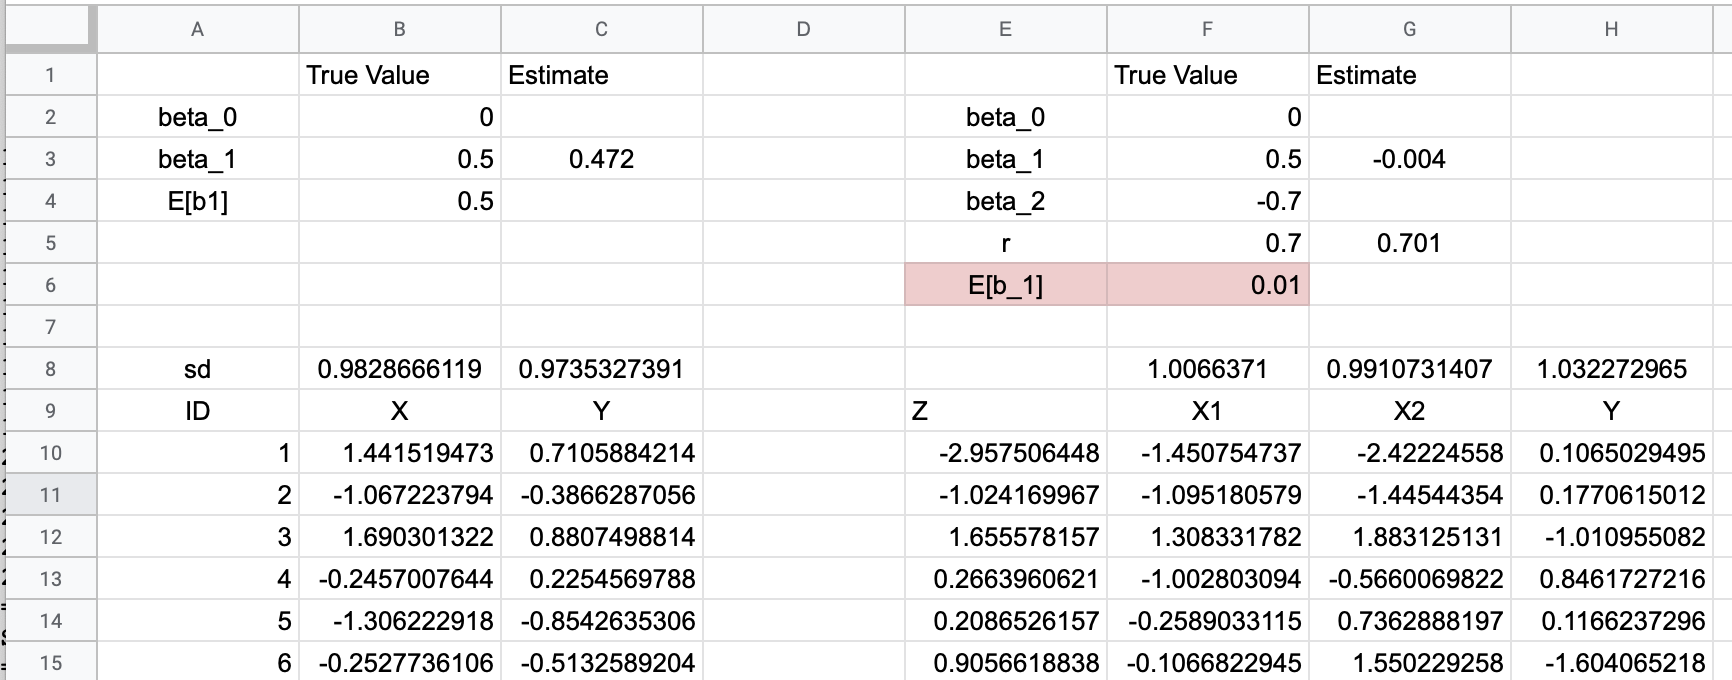
\includegraphics{images/ovb_fig1.png}

\section{Simulation 1}\label{simulation-1}

Open your Google spreadsheet and

\subsection{Step 1. Set up the
parameters}\label{step-1.-set-up-the-parameters}

\begin{enumerate}
\def\labelenumi{\arabic{enumi}.}
\tightlist
\item
  In column A, cells 2-4, insert ``beta\_0'', ``beta\_1'', ``E{[}b1{]}''
  (see figure above)
\item
  In row 1, columns B and C, insert ``True Value'', ``Estimate''
\item
  In B2, insert a number (it doesn't matter)
\item
  In B3, insert 0.5 (this is the true generating effect of X on Y)
\item
  In B4, insert =B3 (this is the expected value of the generating effect
  of X on Y given the statistical model)
\end{enumerate}

\subsection{Step 2. Generate fake
data}\label{step-2.-generate-fake-data}

\begin{enumerate}
\def\labelenumi{\arabic{enumi}.}
\tightlist
\item
  In row 9, coumns A-C, insert ``ID'', ``X'', ``Y''
\item
  In A10 insert ``1''
\item
  In B10 insert \texttt{=normsinv(rand())}
\item
  In C10 insert
  \texttt{=\$B\$2\ +\ \$B\$3*B10\ +\ sqrt(1-\$B\$3\^{}2)*normsinv(rand())}
\item
  In A11 insert \texttt{=A10\ +\ 1}
\item
  Highlight cells B10 and C10. Click on the handle on the lower right
  corner of the box and drag down 1 row. Your formulas from row 10
  should now be in row 11.
\item
  Highlight cells A11, B11, C11. Click on the handle on the lower right
  corner of the box and drag down and down and down until you get to row
  1000. You should have copied all three formuilas all the way down.
\end{enumerate}

What is step 2 doing? It is creating fake data. The value is caused by
three things, the value in Cell B2, the product of B3 and X, and a
random number. The value in B3 is the contribution of X to Y or how ``X
causes Y'' or the ``causal effect of X on Y''. If B3 is 0 then there is
no causal effect. If B3 is 1 or -1, then the random component is zero.

You have just created fake data with a known generating mechanism! But
it is imperative to check the the equations you entered don't have bugs.
If the equations were entered correctly, the standard deviation of the X
and Y columns should both be one. Check this

\subsection{Step 3. Fake data check}\label{step-3.-fake-data-check}

\begin{enumerate}
\def\labelenumi{\arabic{enumi}.}
\tightlist
\item
  In A8, insert ``sd''
\item
  In B8, insert \texttt{=stdev(B10:B1000)}
\item
  Copy B8 and paste in C8.
\end{enumerate}

These numbers should be close to 1.0 (something is probably wrong if it
is less than 0.95 or more than 1.05). Refresh the spread sheet by typing
command-R (Mac) or control-R (Windows)

\subsection{Step 4. Does a statistical model recover the known
effect?}\label{step-4.-does-a-statistical-model-recover-the-known-effect}

\begin{enumerate}
\def\labelenumi{\arabic{enumi}.}
\tightlist
\item
  In C3, insert \texttt{=slope(C10:C1000,\ B10:B1000)}
\item
  In C3, round to three places after the decimal
\end{enumerate}

This is the slope of the regression (the statistical model) of Y on X.
It is the \textbf{estimate} of the causal effect. The number should be
very close to the true value.

This slope is the \textbf{regression coefficient} b1. The cell labeled
``E{[}b1{]}'' is the ``expectation of b1'' or the expected value of b1.
Your estimate of beta\_1 should also be very close to E(b1) since E(b1)
is equal to the true generating effect (beta\_1).

\subsection{What you did}\label{what-you-did}

\subsubsection{\ldots{} in a nutshell}\label{in-a-nutshell}

you generated \(Y\) using a ``data generating'' mechanism and then using
the available data (X and Y), you used a statistical analysis to see if
you could recover this data generating mechanism. The data generating
mechanism is the set of two coefficients \(\beta_0\) and \(\beta_1\).

\subsubsection{the data generating mechaniusm in a little more
detail}\label{the-data-generating-mechaniusm-in-a-little-more-detail}

The fake data are two variables, X and Y. Y is caused by three things:

\begin{equation}
y_i = \beta_0 + \beta_1 x_i + \sigma_i
\end{equation}

the subscript is the ``\(i\)th'' individual (if ID=7 then i=7). The
three components generating \(y_i\) are

\begin{enumerate}
\def\labelenumi{\arabic{enumi}.}
\tightlist
\item
  \(\beta_0\) is ``the intercept''; it is common to all \(i\)
\item
  \(\beta_1 x_i\) is the product of the effect (\(\beta_1\)) and an
  individuals value of \(x\). \(\beta_1\) is the same for all \(i\) but
  the product is unique to each \(i\).
\item
  \(\sigma_i\) is ``the error''; this is the random variation due to
  other factors that ``cause'' Y but are unique to each \(i\). That is,
  these factors are \textbf{not correlated} with \(X\).
\end{enumerate}

\subsection{The model you fit is}\label{the-model-you-fit-is}

\begin{equation}
y_i = b_0 + b_1 x_i + e_i
\end{equation}

\begin{enumerate}
\def\labelenumi{\arabic{enumi}.}
\tightlist
\item
  \(b_0\) is the intercept
\item
  \(b_1\) is the slope
\item
  \(e_i\) is the residual (the difference between the modeled value and
  the actual value)
\end{enumerate}

Notice that the statistical model is the same as the generating model.
It is not at all surprising that the statistical model ``recovers'' the
data generating mechanism (or the ``true values''). \textbf{The problem
in science is, we don't know the data generating model so we don't know
the correct statistical model}. This will hopefully make more sense in
the next exercise.

\section{Simulation 2}\label{simulation-2}

\subsection{Step 5. Set up the
parameters}\label{step-5.-set-up-the-parameters}

\begin{enumerate}
\def\labelenumi{\arabic{enumi}.}
\tightlist
\item
  In column E, rows 2-6, insert the labels ``beta\_0'', ``beta\_1'',
  ``beta\_2'', ``r'', ``E(b\_1)''
\item
  In row 1, columns F and G, insert the labels ``True Value'',
  ``Estimate''
\item
  In F2, insert a number (it doesn't matter) (this is the baseline value
  of generating model)
\item
  In F3, insert 0.5 (this is the true generating effect of \(X_1\) on Y)
\item
  In F4, insert -0.7 (this is the true generating effect of \(X_2\) on
  Y)
\item
  In F5, insert 0.7 (this is the true correlation between \(X_1\) and
  \(X_2\))
\end{enumerate}

\subsection{Step 6. Generate fake
data}\label{step-6.-generate-fake-data}

\begin{enumerate}
\def\labelenumi{\arabic{enumi}.}
\tightlist
\item
  In row 9, coumns E-H, insert ``Z'', ``X1'', ``X2'', ``Y''
\item
  In E10 insert \texttt{=normsinv(rand())}
\item
  In F10 insert
  \texttt{=sqrt(\$F\$5)*\$E10\ +\ sqrt(1-\$F\$5)*normsinv(rand())}
\item
  In G10, copy the equation from F10 and insert into G10
\item
  In H10, insert
  \texttt{=\$F\$2\ +\ \$F\$3*F10\ +\ \$F\$4*G10\ +\ sqrt(1-\$F\$3\^{}2\ -\ \$F\$4\^{}2\ -\ 2*\$F\$3*\$F\$4*\$F\$5)*normsinv(rand())}
\item
  Highlight cells E10 through H10. Click on the handle on the lower
  right corner of the box and drag down and down and down until you get
  to row 1000. You should have copied all four formuilas all the way
  down.
\end{enumerate}

What is step 6 doing? Like Step 2 in Simulation 1 above, it is creating
fake data. But here the \(Y\) value is caused by five things:

\begin{equation}
y_i = \beta_0 + \beta_1 x_{1i} + \beta_2 x_{2i} + \sigma_i
\end{equation}

\begin{enumerate}
\def\labelenumi{\arabic{enumi}.}
\tightlist
\item
  \(\beta_0\) is ``the intercept''; it is common to all \(i\)
\item
  \(\beta_1 x_{1i}\) is the product of the effect (\(\beta_1\)) and an
  individuals value of \(x_1\). \(\beta_1\) is the same for all \(i\)
  but the product is unique to each \(i\). This is the causal or
  generating effect of \(X_1\) on \(Y\)
\item
  \(\beta_2 x_{2i}\) is the product of the effect (\(\beta_2\)) and an
  individuals value of \(x_2\). \(\beta_2\) is the same for all \(i\)
  but the product is unique to each \(i\). This is the causal or
  generating effect of \(X_2\) on \(Y\)
\item
  \(\sigma_i\) is ``the error''; this is the random variation due to
  other factors that ``cause'' \(Y\) but are unique to each \(i\). That
  is, these factors are \textbf{not correlated} with \(X\).
\end{enumerate}

what is the 5th cause of \(Y\)?

\begin{enumerate}
\def\labelenumi{\arabic{enumi}.}
\setcounter{enumi}{4}
\tightlist
\item
  \(r\) -- the correlation between \(X_1\) and \(X_2\). A correlation is
  a measures of association and is always between -1 and 1
\end{enumerate}

\subsection{Step 7. Fake data check}\label{step-7.-fake-data-check}

\begin{enumerate}
\def\labelenumi{\arabic{enumi}.}
\tightlist
\item
  Check the standard deviation of \(X_1\), \(X_2\), and \(Y\) as in Step
  3 above. All of these should be close to 1.0
\item
  insert \texttt{=correl(F10:F1000,\ G10:G1000)} in G5. This should be
  close to the true correlation in F5 (The starting correlation is 0.7,
  so the estimate should be 0.67-0.73)
\end{enumerate}

\subsection{Step 8. Does a statistical model recover the known
effect?}\label{step-8.-does-a-statistical-model-recover-the-known-effect}

\begin{enumerate}
\def\labelenumi{\arabic{enumi}.}
\tightlist
\item
  In G3, insert \texttt{=slope(H10:H1000,\ F10:F1000)}
\item
  In G3, round to three places after the decimal
\end{enumerate}

As in Step 4 in Siumulation 1 above, this is the slope of the regression
(the statistical model) of \(Y\) on X. It is the \textbf{estimate} of
the causal effect. The number will not be very close to the true
generating value (\(\beta_1\)), at least using the default values
specified in Step 5. But it should be close to E(b1) (the expected value
of b1), given the statistical model. But, unlike simulation 1, E(b1) is
not similar to \(\beta_1\), the true generating effect. Huh?

\begin{enumerate}
\def\labelenumi{\arabic{enumi}.}
\tightlist
\item
  E(b1) should not equal the true value of beta\_1 (at least using
  default values in Step 5), unlike in Simulation 1.
\item
  Your estimate of beta\_1 should be very close to E(b1) but not to
  beta\_1
\end{enumerate}

\subsection{What's going on is the whole point of this
exercise}\label{whats-going-on-is-the-whole-point-of-this-exercise}

You have measured \(Y\) and \(X_1\) but have not measured \(X_2\).
Because you haven't measured \(X_2\), it is \emph{not} in your
statistical model, so your statistical model is just like that in
Simulation 1.

\begin{equation}
y_i = b_0 + b_1 x1_i + e_i
\end{equation}

But the generating model for \(Y\) is

\begin{equation}
y_i = \beta_0 + \beta_1 x_{1i} + \beta_2 x_{2i} + \sigma_i
\end{equation}

That is, your statistical model has an \textbf{omitted causal variable}
(\(X_2\)) and your estimate of the effect of \(X_1\) is \textbf{biased}.
This kind of bias is called \textbf{omitted variable bias}. The true
effect of \(X_1\) on \(Y\) is \(\beta_1\) but you are actually
estimating E(b1) with the regression coefficient! Researchers often
think their result will get closer to the truth as the sample size
increases but if an causal effect is missing from a statistical model,
the estimate of the effects of the factors in the model will never ever
get closer to the truth - instead it gets closer to the wrong thing (the
biased expectation of the effect given the model).

\section{Questions}\label{questions}

\subsection{Simulation 1}\label{simulation-1-1}

\begin{enumerate}
\def\labelenumi{\arabic{enumi}.}
\tightlist
\item
  Given the default parameters specified above, what is the estimated
  effect of \(X_1\) on \(Y\) in Simulation 1?
\item
  What is the true effect of \(X_1\) on \(Y\) in Simulation 1?
\item
  If you increase your sample size, will the estimated effect of \(X_1\)
  on \(Y\) move toward the true effect of \(X_1\) on \(Y\) in Simulation
  1?
\end{enumerate}

\subsection{Simulation 2}\label{simulation-2-1}

\begin{enumerate}
\def\labelenumi{\arabic{enumi}.}
\setcounter{enumi}{3}
\tightlist
\item
  Given the default parameters specified above, what is the estimated
  effect of \(X_1\) on \(Y\) in Simulation 2?
\item
  What is the true effect of \(X_1\) on \(Y\) in Simulation 2?
\item
  If you increase your sample size, will the estimated effect of \(X_1\)
  on \(Y\) move toward the true effect of \(X_1\) on \(Y\) in Simulation
  2?
\item
  If you did a study of \(X_1\) on \(Y\) and the true generating model
  of \(Y\) is that in Simulation 2, what would you conclude about the
  effect of \(X_1\) on \(Y\)?
\end{enumerate}

\subsection{Simulation 2 with new
parameters}\label{simulation-2-with-new-parameters}

Redo Simulation 2 with the parameters: \(\beta_1 = 0.0\). Leave
\(\beta_2 = -0.7\) and \(r=0.7\).

\begin{enumerate}
\def\labelenumi{\arabic{enumi}.}
\setcounter{enumi}{7}
\tightlist
\item
  What is the estimated effect of \(X_1\) on \(Y\)?
\item
  What is the true effect of \(X_1\) on \(Y\) in Simulation 2?
\item
  If you did a study of \(X_1\) on \(Y\) and the true generating model
  of \(Y\) is these new parameters in Simulation 2, what would you
  conclude about the effect of \(X_1\) on \(Y\)?
\end{enumerate}

\chapter{Metabolism}\label{metabolism}

\chapter{Physiological Genetics}\label{physiological-genetics}

\chapter{Cancer}\label{cancer}

\bibliography{book.bib,packages.bib}


\end{document}
